\documentclass{article}
\usepackage{amsmath, amssymb, cite, algorithmic, url, braket}
\usepackage{graphicx}
\usepackage{pythonhighlight}
\usepackage[margin=1.5cm]{geometry}
\usepackage[title]{appendix}
\usepackage{subfigure}
\usepackage{listings}
\usepackage{booktabs}
\usepackage{hyperref}

\graphicspath{{../pic/}}
\lstset{
language=[ANSI]{C},
showtabs=true,
tab=,
tabsize=2,
basicstyle=\ttfamily\footnotesize,%\setstretch{.5},
stringstyle=\color{stringcolour},
showstringspaces=false,
alsoletter={1234567890},
otherkeywords={\%, \}, \{, \&, \|},
keywordstyle=\color{keywordcolour}\bfseries,
upquote=true,
morecomment=[s]{/*}{*/},
commentstyle=\color{commentcolour}\slshape,
literate=*%
{=}{{\literatecolour=}}{1}%
{-}{{\literatecolour-}}{1}%
{+}{{\literatecolour+}}{1}%
{*}{{\literatecolour*}}{1}%
{!}{{\literatecolour!}}{1}%
{[}{{\literatecolour[}}{1}%
{]}{{\literatecolour]}}{1}%
{<}{{\literatecolour<}}{1}%
{>}{{\literatecolour>}}{1}%
% {>>>}{\pythonprompt}{3}%
,%
frame=trbl,
rulecolor=\color{black!40},
backgroundcolor=\color{white},
breakindent=.5\textwidth,frame=single,breaklines=true
}

\begin{document}
\title{DSP Homework}
\author{Xu, Minhuan}
\maketitle
\tableofcontents
\begin{abstract}
In the first section I summarized the 2 videos we watched this week, and came up with my opinions. In the second section, I explore the properties of FIR and IIR, and found out in which condition the digital	filters will be stable. In the third section, I drew 3 spectrum to compare with each other in order to find the secret of nice sounds.
\end{abstract}

\section{Videos}
\subsection{Carbon Nanotube}
The video first introduces the structural characteristics of Carbon Nanotube, and compares Carbon Nanotube with diamonds and graphite. Diamond is a regular tetrahedron with three-dimensional structure, which makes diamond obtain very solid physical properties; At the same time, the graphite is a plane hexagon structure. Although it is very strong horizontally, the layered structure is not firm, and the upper and lower layers will slide, which is why the graphite is very soft and slippery. However, the structure of Carbon Nanotube is vividly expressed in the video. That is, the horizontal graphite molecular structure is combined from both sides to form a tubular structure, which greatly improves the physical properties of this material and greatly increases the tensile resistance.

At the same time, the video also introduces the different applications of Carbon Nanotube, because of its good conductivity, it can be used in electric energy transportation; Because of its bio compatible characteristics, it is very suitable for being a natural interface material.

\subsection{Audio Mixer}
This video mainly introduces the specific usage of Audio Mixer. The specific features and functions of this Audio Mixer mainly include: mixing music from multiple channels to send it to the lower level amplifier; Control the loudness of each channel, that is, the amplitude; Power supply for peripheral equipment; Use filter for signal; Adjust the signal strength on different frequency bands.

\subsection{My Thoughts}
\subsubsection*{Carbon Nanotube}
Materials like Carbon Nanotube are very cutting-edge future materials, and also an interesting material close to our information science. I can see the emergence of carbon fiber materials on many futuristic vehicles, such as supercars, Formula 1, etc.

This video, which starts with the basic theory, reminds me of my chemistry knowledge in senior high school. Even though I have not involved any knowledge about senior high school chemistry in my college life for more than two years, it does not mean that my professional field has no connection with other traditional engineering subjects.

\subsubsection*{Audio Mixer}
Just as we found the application of other disciplines in the information field in the last video, this Audio Mixer is an example of the brilliant performance of information disciplines in other fields. In fact, we have found that music and signal processing are inseparable in modern times through the study of signal processing courses. In the information age, more and more media containing information have changed from letters to current electromagnetic waves or electrical signals transmitted in circuits.

This makes me think that in fact, there is a certain amount of signal transmission in the mouse, headset, monitor, and even charger that we often use. Electrical signals are everywhere, so we must be careful.


\section{FIR And IIR}
\subsection{Digital Filter System}
\subsubsection{When Q is equal to 0}
When $Q = 0$, the system can be represented as 
$$
y(n) = a_0x(n) + \cdots + a_Px(n - P)
$$
Then, the $h(n)$ can be written as
$$
h(n) =  \sum_i^P a_i \times \delta(n - i)
$$
So, $h(n)$ has finite duration, the system is FIR.
\subsubsection{When Q is greater than 0}
When $Q > 0$, the system can be represented as 
\begin{equation}
y(n) + b_1 y(n - 1) + \cdots + b_Q y(n - Q) = a_0 x(n) + a_1 x(n - 1) + \cdots + a_P x(n - P)
\label{eq:iir}
\end{equation}
We can know that the $y(n), y(n - 1), y(n - 2), \cdots $ is 
\begin{gather}
y(n) = a_0 x(n) + a_1 x(n - 1) + \cdots + a_P x(n - P) - b_1 y(n - 1) - \cdots - b_Q y(n - Q) \label{eq:yn} \\ 
y(n - 1) = a_0 x(n - 1) + a_1 x(n - 2) + \cdots + a_P x(n - P - 1) - b_1 y(n - 2) - \cdots - b_Q y(n - Q - 1) \label{eq:yn-1} \\ 
y(n - 2) = a_0 x(n - 2) + a_1 x(n - 3) + \cdots + a_P x(n - P - 2) - b_1 y(n - 3) - \cdots - b_Q y(n - Q - 2) \label{eq:yn-2} \\ 
y(n - 3) = a_0 x(n - 3) + a_1 x(n - 4) + \cdots + a_P x(n - P - 3) - b_1 y(n - 4) - \cdots - b_Q y(n - Q - 3) \notag \\ 
\cdots \notag
\end{gather}

Equation (\ref{eq:yn}) contains all the terms in (\ref{eq:yn-1}), and (\ref{eq:yn-1}) contains all the terms in (\ref{eq:yn-2}), all the same below, so (\ref{eq:yn}) seems to have more terms than (\ref{eq:yn-1}). However, actually there are always the same number of terms in each equation, so (\ref{eq:yn}) does contain all the terms in (\ref{eq:yn-1}), but also it has the same number of terms compared with the equations below. Only possibility is that $y(n)$ and $y(n - 1)$ and so on have infinite number of terms. In one word, the system which (\ref{eq:iir}) reveals is IIR.
\subsection{Stability}
\subsubsection{Digital Filter Stability}
When a digital filter has the feature that when input is bounded, the output must be bounded, this digital filter is stable.
\subsubsection{FIR Stability}
FIR can be expressed as below
$$
y(n) = a_0x(n) + \cdots + a_Px(n - P)
$$
If $x(n)$ is bounded, we can always find a maximum of $|x(n)|$ which we call it $max\{ |x| \}$. And we can find the maximum of $|a_i|$ which we call it $A$ as well. So

\begin{align*}
y(n)  &= a_0x(n) + \cdots + a_Px(n - P) \\ 
&< |a_0||x(n)| + \cdots + |a_P||x(n - P)| \\ 
&< A\times max\{ x \} \times P \\ 
&< \infty
\end{align*}

\subsubsection{IIR Stability}
We have
\begin{align*}
	|y(n)| &= |x(n) * h(n)| \\ 
	& \leq \sum_{m} |x(m) \times h(m - n)| \\ 
	& \leq \sum_{m} |x(m)| \times |h(n - m)| \\ 
	& \leq \sum_{m} max\{ |x| \} \times h(n - m) \\ 
	& = max\{ |x| \}  \sum_{m} h(m)
\end{align*}
and if we need $y(n) < \infty$, we should have
\begin{equation}
\sum_{- \infty}^{\infty} h(n) < \infty
\label{eq:limit}
\end{equation}

Look at the $\tilde{h}(z)$ which we can get from (\ref{eq:yn}):
\begin{equation}
	\tilde{h}(z) = \frac{\sum_{p = 0}^{P}a_p z^{-p}}{\sum_{q = 0}^{Q} b_q z^{-q}}
	\label{eq:hz}
\end{equation}

According to mathematics, we can rewrite $h(z)$ as below. The $z^{\lambda-1}$ in the coefficient only represents time-delay. In this condition, we don't care about it

\begin{equation}
\tilde{h}(z) = z^{\lambda - 1} \left[ \frac{z}{z - \alpha_0} + \frac{z}{z - \alpha_1 } + \cdots + \frac{z}{z - \alpha_N } \right]
\label{eq:hzz}
\end{equation}

First, we know, in frequency domain, the $\frac{z}{z - \alpha} = \frac{1}{1 - \alpha/z} = \sum_{- \infty}^{\infty} az^{-1}$ means $\alpha^n$ in time domain.

Second, see (\ref{eq:hzz}) again, and in order to satisfy the requirement in (\ref{eq:limit}), we need to make all poles in (\ref{eq:hzz}) (which are $\alpha$ here) less than $1$, so that all $\alpha^n$ will converge, at last $h(z)$ will also converge.

\subsubsection{An Example in Class}
When $Q = 2, P = 0$, we have

\begin{equation}
y(n) + b_1y(n - 1) + b_2y(n - 2) = a_0 x(n)
\label{eq:yxExample}
\end{equation}
In this condition, $\tilde{h}(z)$ is like 
\begin{equation}
\tilde{h}(z) = \frac{a_0}{1 + b_1 z^{-1} + b_2 z^{-2}} = \frac{a_0 z^2}{z^2 + b_1 z + b_2}
\label{eq:hzExample}
\end{equation}
Here, the expression of $H(z)$ is as below
\begin{equation}
H(z) = z^2 + b_1 z + b_2
\label{eq:Hz}
\end{equation}
Roots of this equation is $z = -b_1 \pm \sqrt{b_1^2 - 4 b_2}$.

\paragraph{Real Roots}
First, if (\ref{eq:Hz}) has real root(s), to make the root(s) be in (-1, 1), the sufficient and necessary conditions is as below
\begin{equation}
	\begin{aligned}
		\begin{cases}
			H(-1) = 1 - b_1 + b_2 > 0 \\ 
			H(1) = 1 + b_1 + b_2 > 0 \\ 
			- \frac{b_1}{2} \in (-1, 1)
		\end{cases}
	\end{aligned}
	\label{eq:realRoot}
\end{equation}
It is easy using linear programming to prove that all the conditions above can be derived from $|b_1| + |b_2| < 1$, or in mathematics, $|b_1| + |b_2| < 1 \Rightarrow (\ref{eq:realRoot})$.

\paragraph{Complex Roots}
Second, if (\ref{eq:Hz}) has complex root(s), to make the root(s) be in (-1, 1), the sufficient and necessary conditions is as below

\begin{align*}
		|\alpha_1| = |\alpha_2| &= |\frac{-b_1 \pm j\sqrt{4b_2 - b_1^2}}{2}| \\ 
		&= \sqrt{b_2} \in (-1, 1)
\end{align*}
It is easy to find that $|b_1| + |b_2| < 1 \Rightarrow \sqrt{b_2} \in (-1, 1)$. 

In conclusion, we can find that if $|b_1| + |b_2| < 1$ is true, the roots of $H(z)$ is all within the unit circle which means the system in (\ref{eq:hz}) is stable. So, $|b_1| + |b_2| < 1$ is a sufficient condition for the IIR system to be stable when $Q = 2, P = 0$.

\section{Why Some Voices Sound nicer}
\subsection{Harmonic Series}
I have 3 sounds here, they're all from a video\cite{harmonicSeries} which I watched the other day. Look at the spectrum of them below in Fig.~\ref{fig:spectrumComparison}. Respectively, here are the frequency spectrum of piano, cello and vocal voice (from left to right) making sounds of the same pitch (the same fundamental wave). Actually, the lowest frequency is $130~ \mathrm{Hz}$, and the other frequency are just the integer multiples. We learned the harmonic series in physics lessons, this spectrum is a good reflection of this knowledge point. 

\subsection{Reason}
Back to the topic, we can tell the sound is nice or not, in this condition, I think the piano is nicer than this man's voice. According to the spectrum, the only notable difference is that the \emph{ratio} between different harmonic series. For example, in piano's record, second harmonic is the highest in the spectrum which mean it has the biggest amplitude among the harmonic series. However, in violin's record, third harmonic is the biggest.

So, if a sound sounds nice, that means the radio between different harmonic series \emph{looks} nice.

\begin{figure}[!h]
	\centering
	\subfigure[Piano]{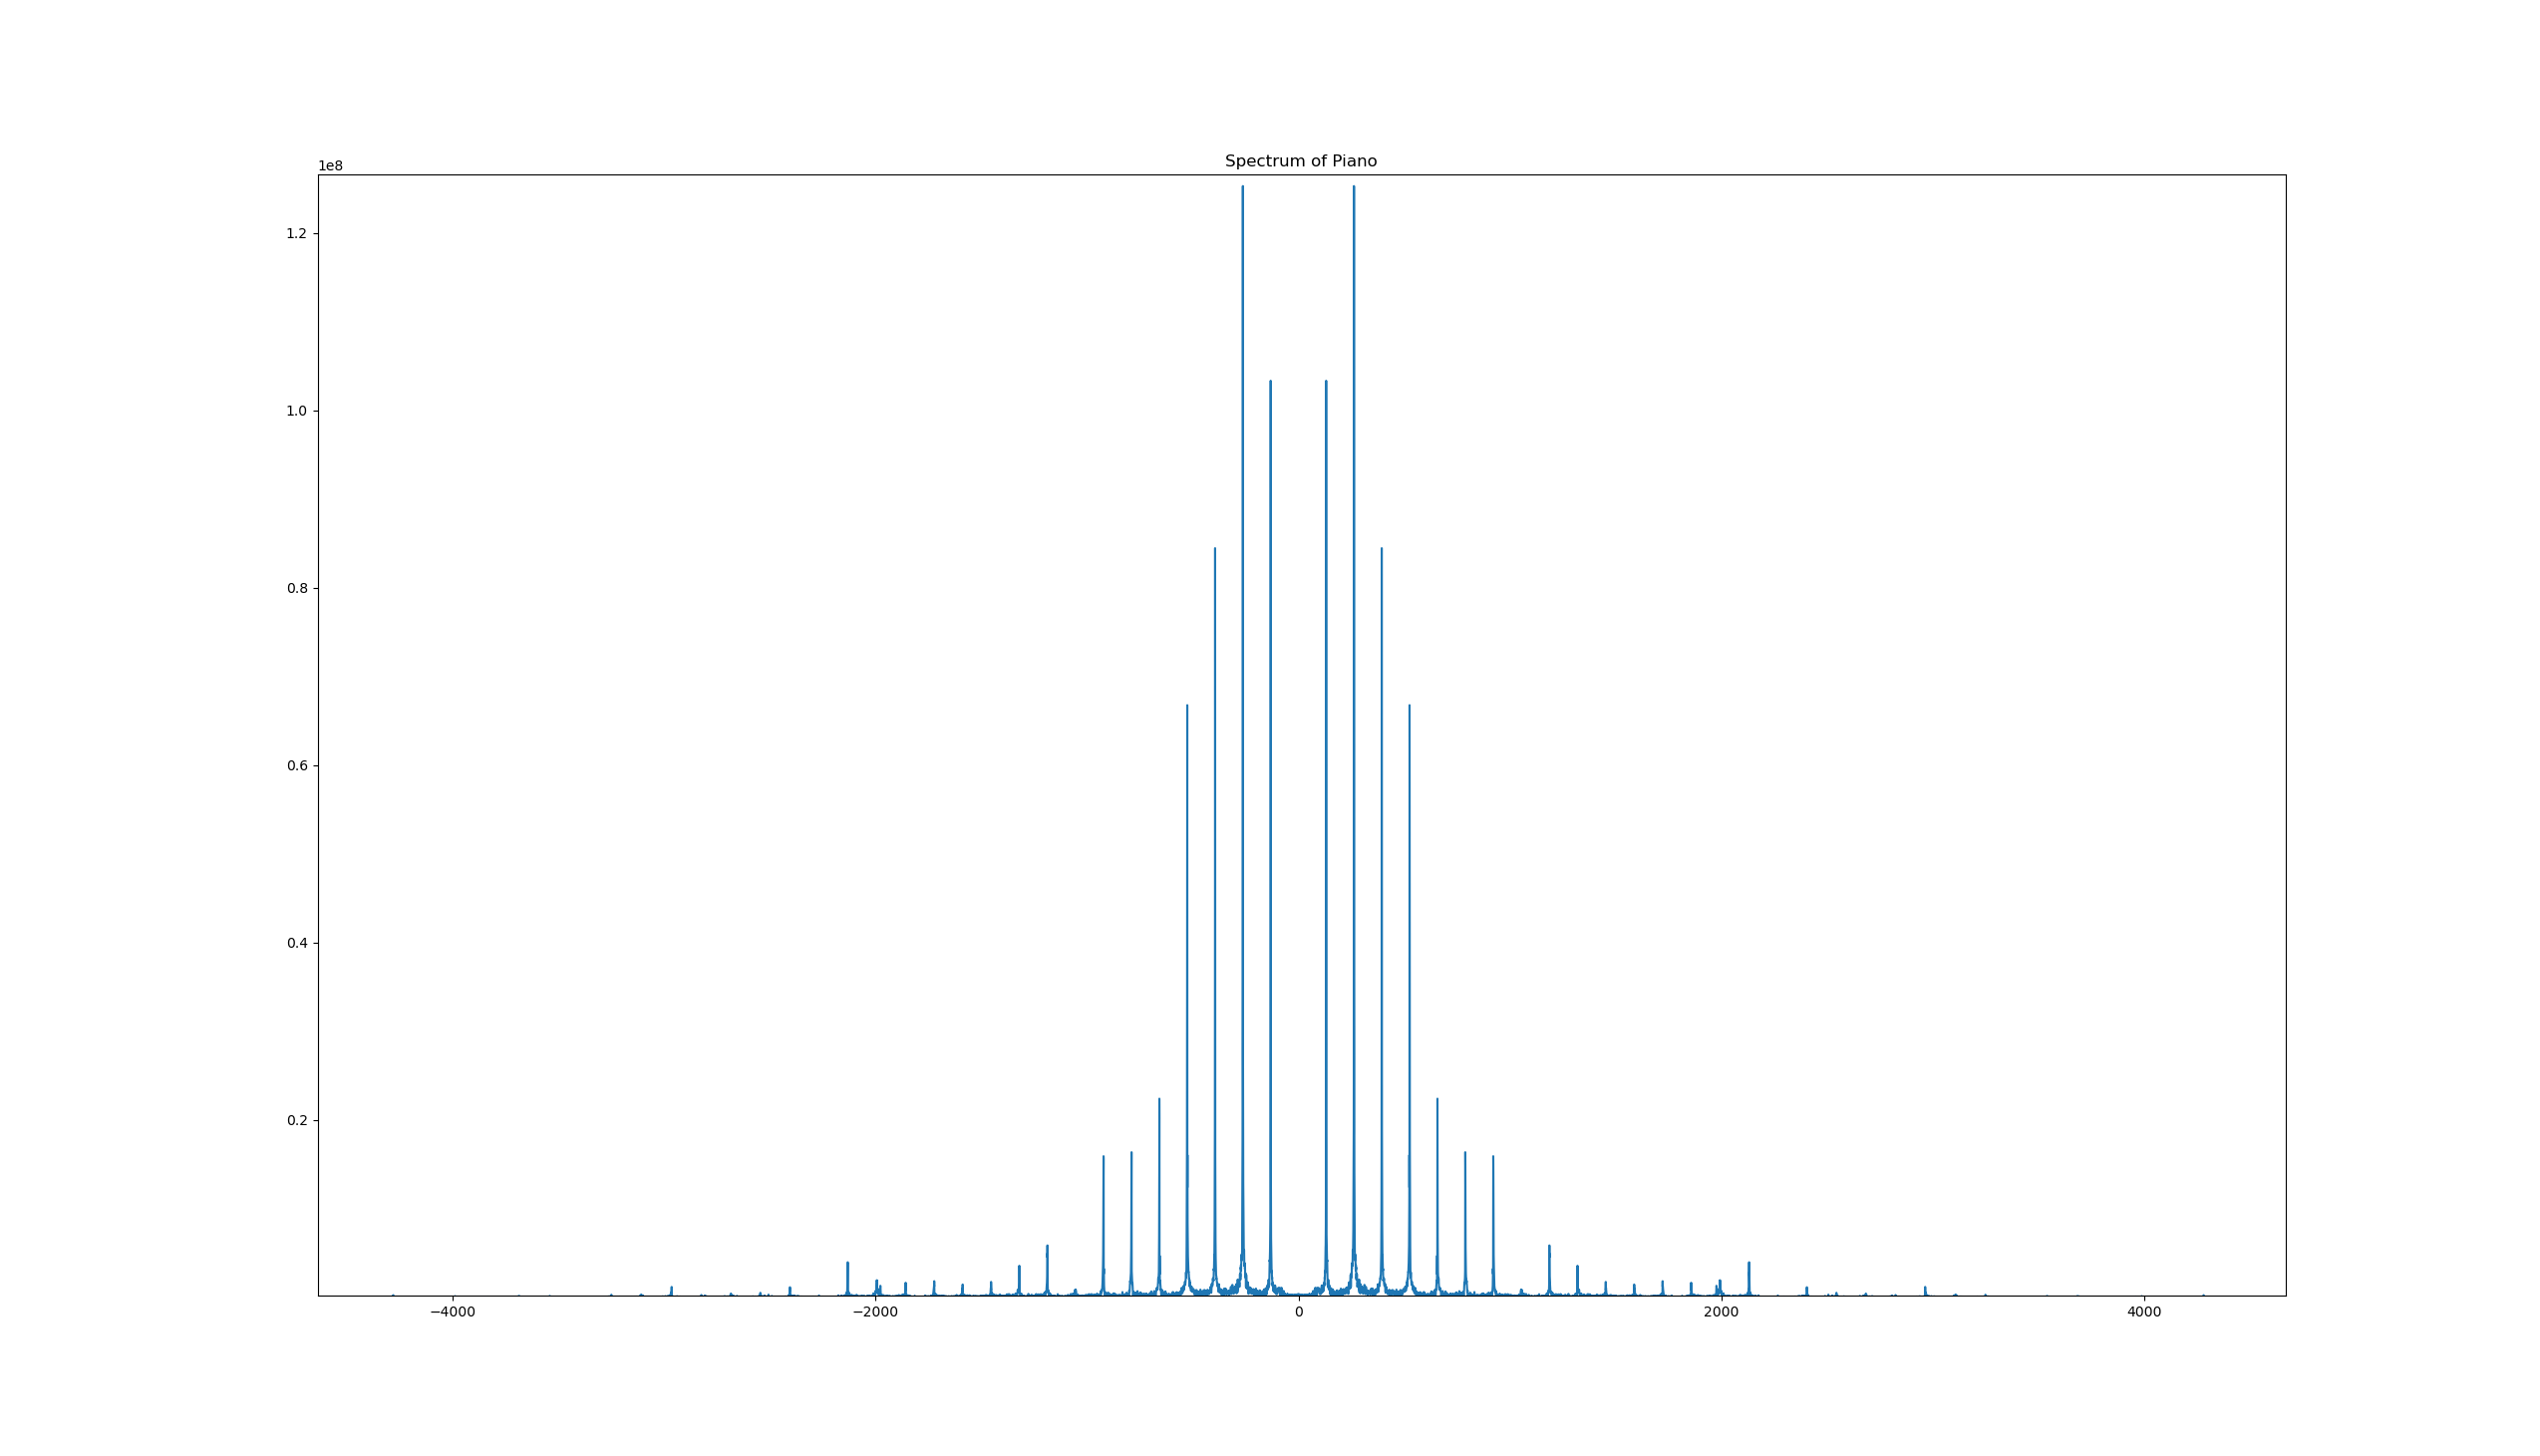
\includegraphics[height=1.3 in]{../pic/SpectrumOfPiano.png}}
	\hspace{0 pt}
	\subfigure[Cello]{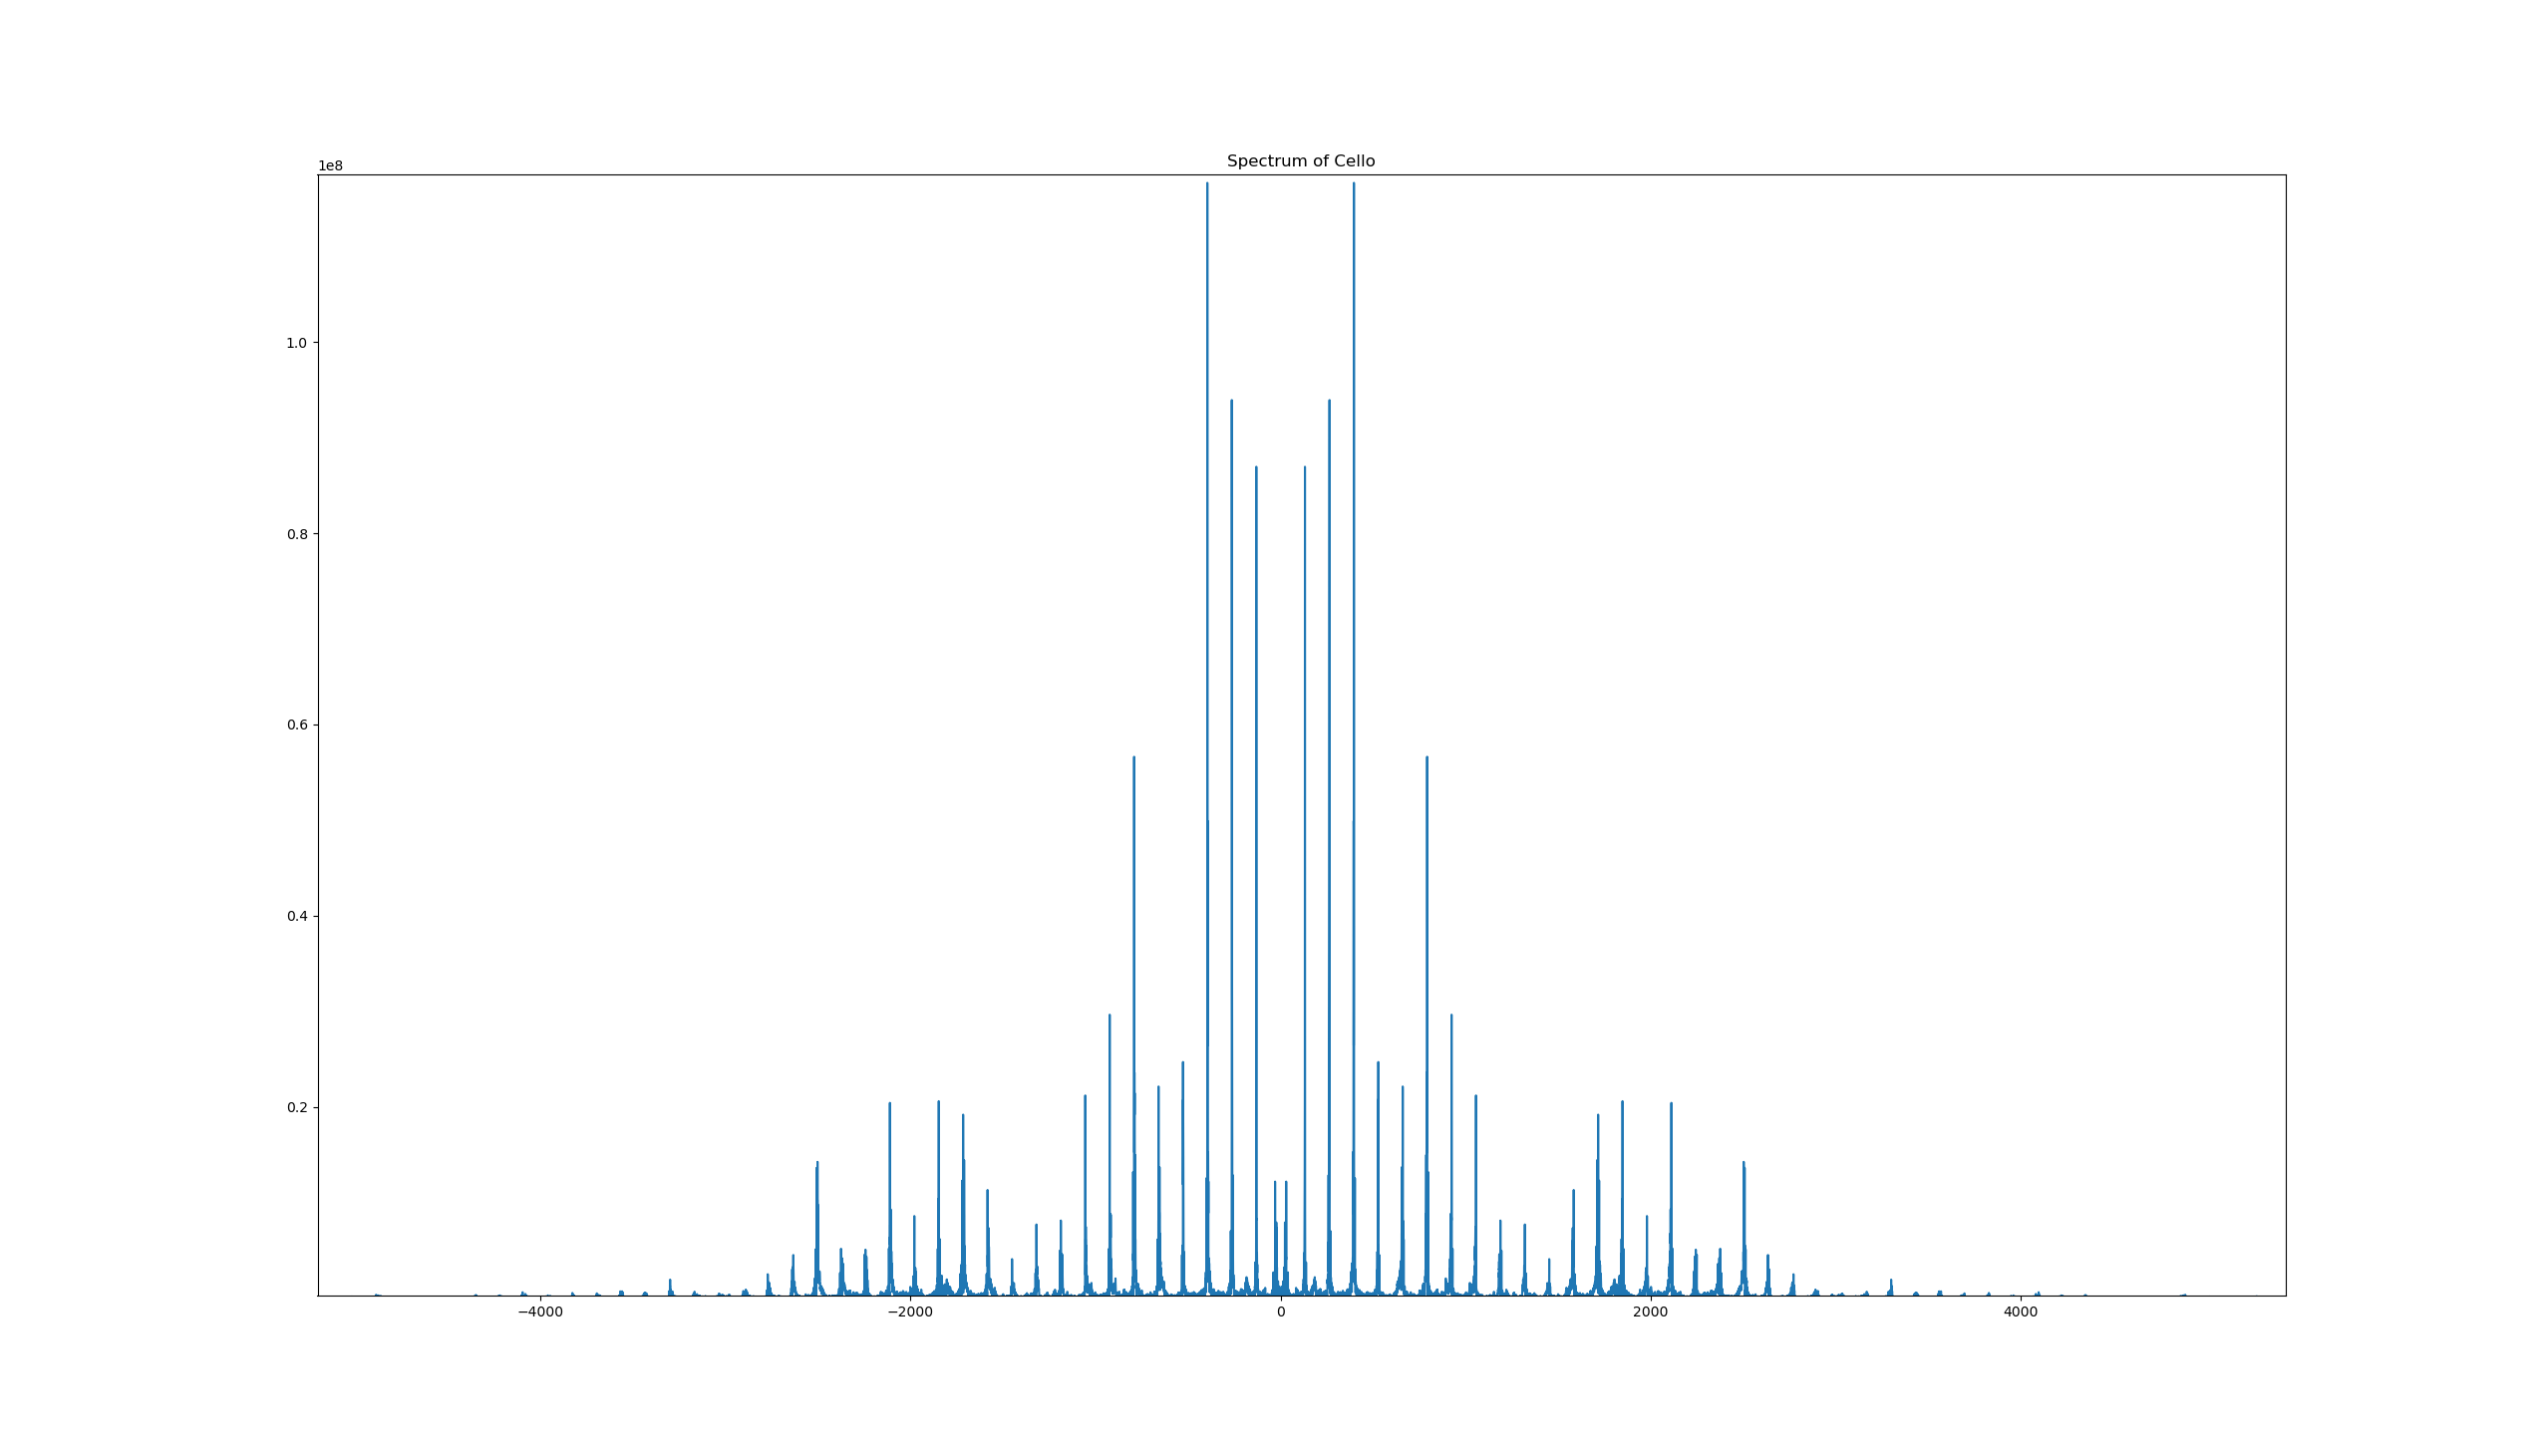
\includegraphics[height=1.3 in]{../pic/SpectrumOfCello.png}}
	\hspace{0 pt}
	\subfigure[Man]{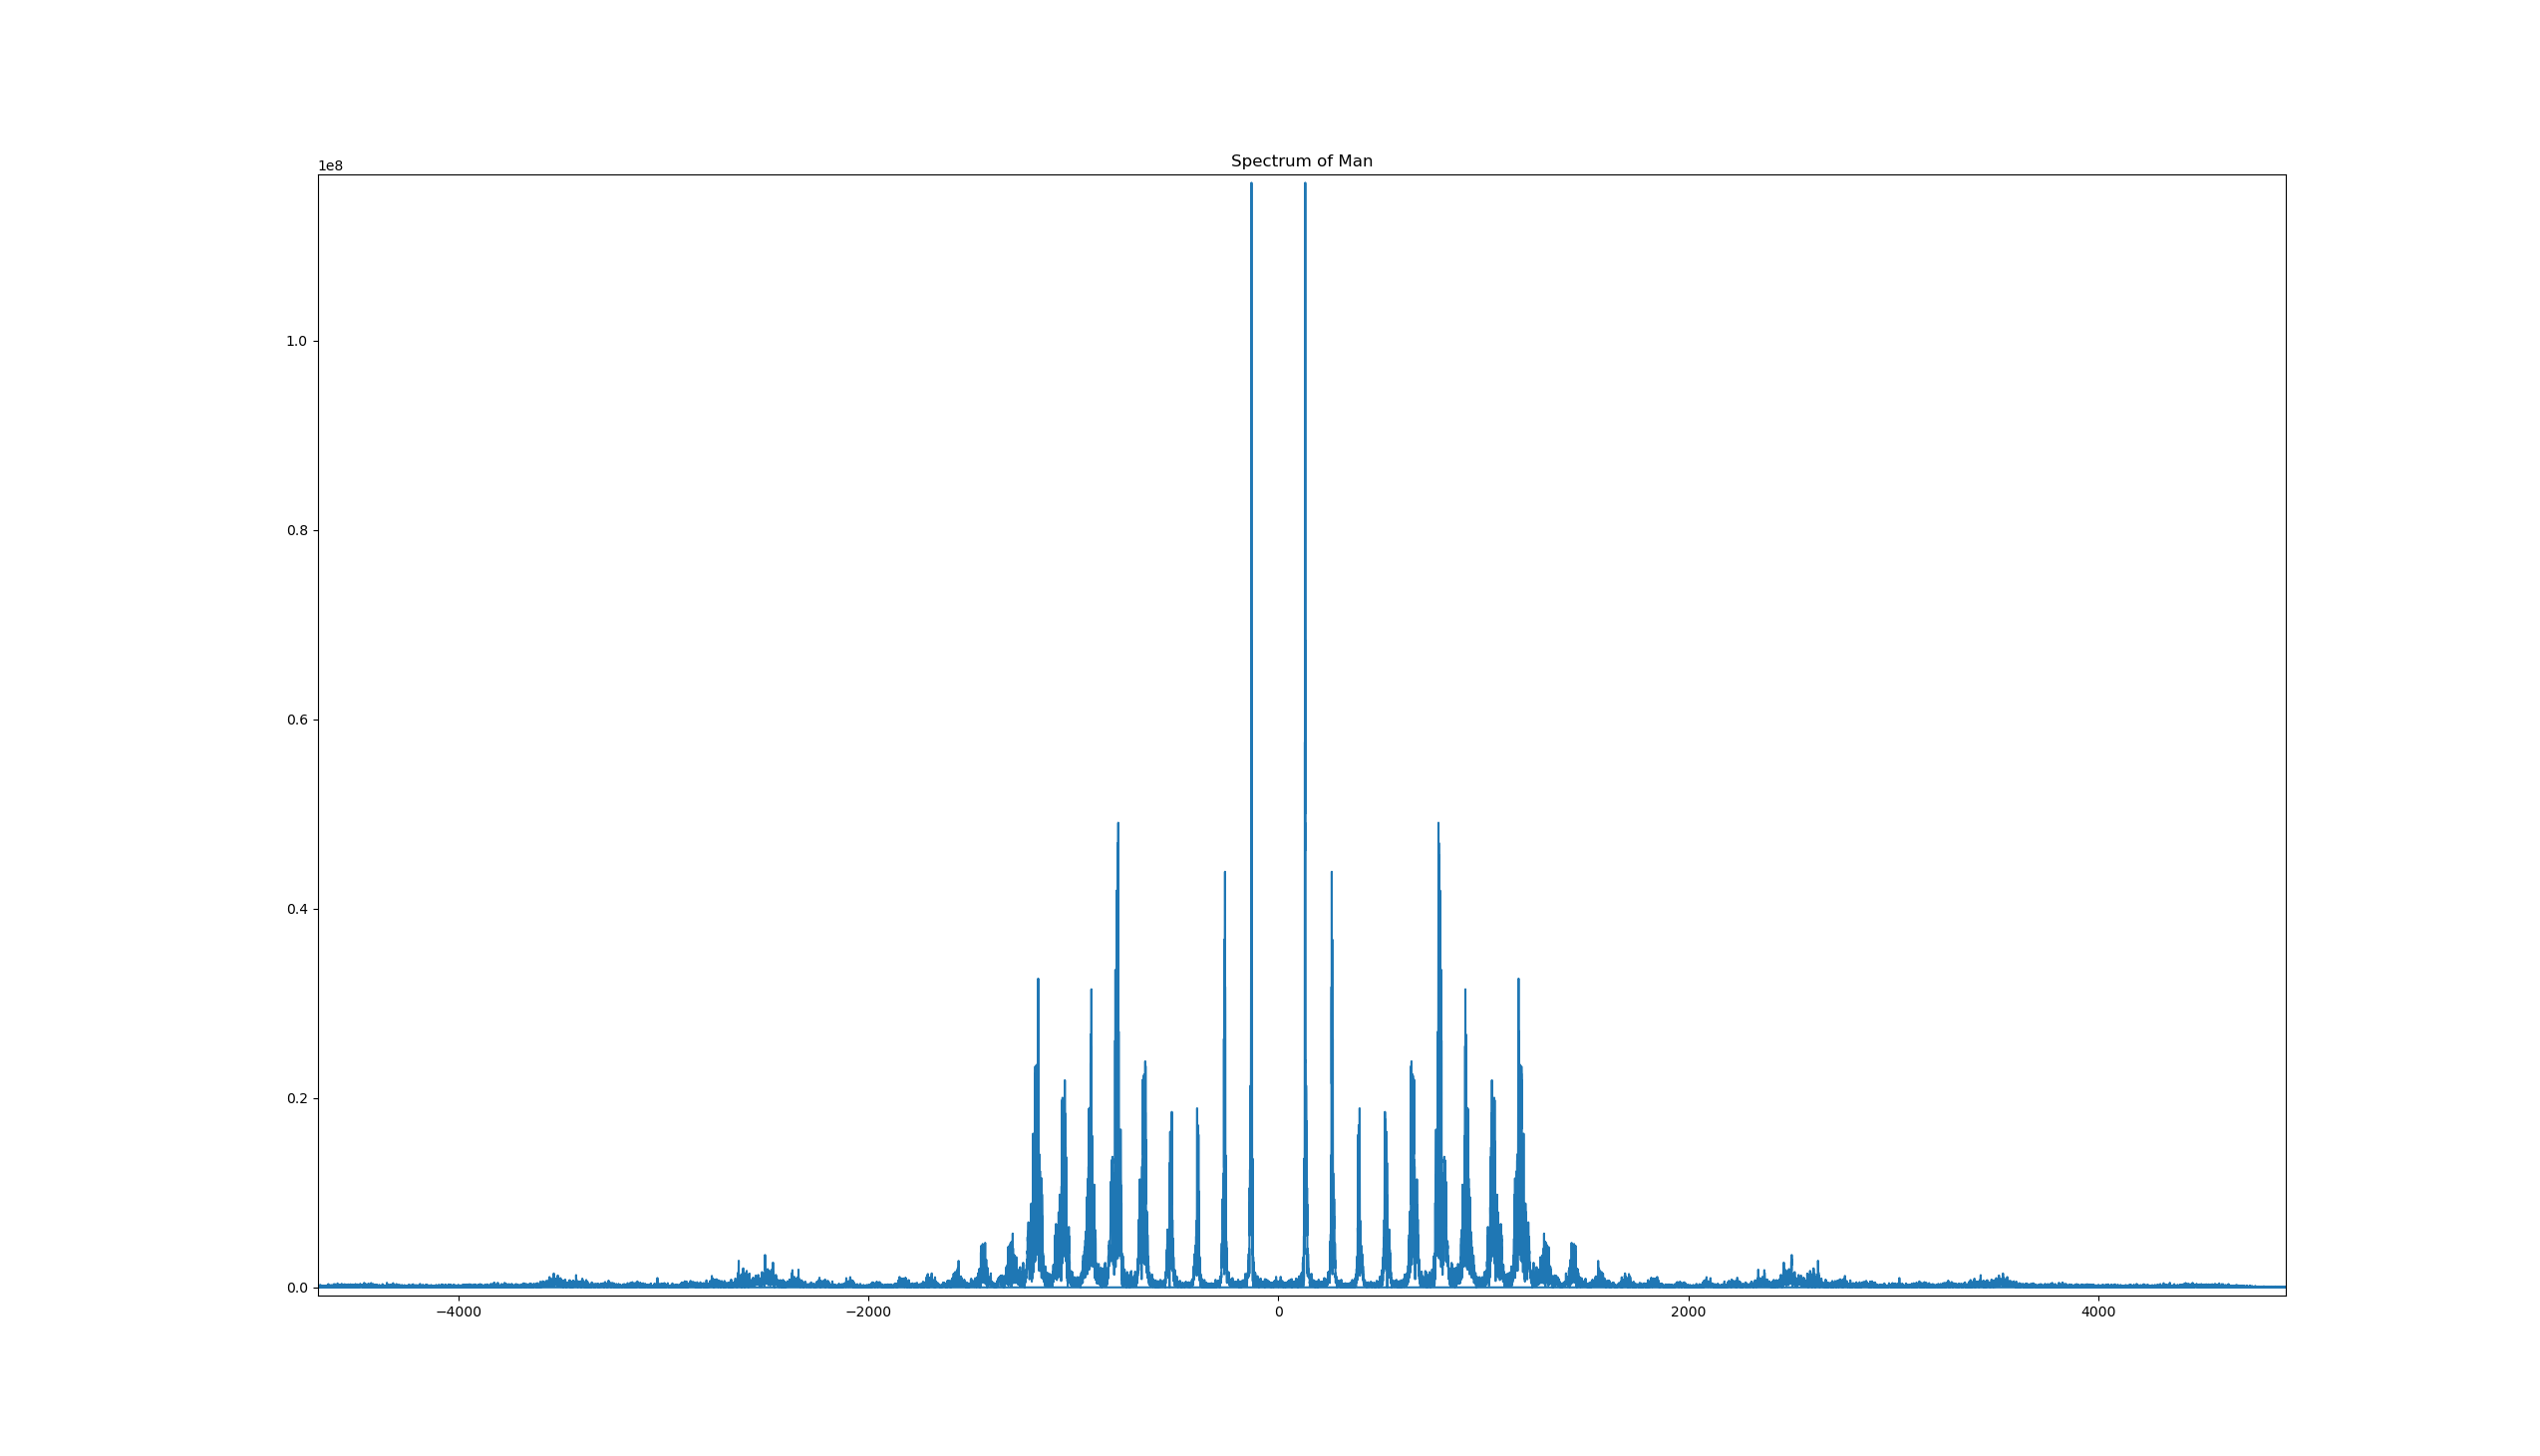
\includegraphics[height=1.3 in]{../pic/SpectrumOfMan.png}}
	\caption{Spectrum Of different Sounds}
	\label{fig:spectrumComparison} 
\end{figure}

\newpage


\bibliographystyle{ieeetr}
\bibliography{../bib/database}

\begin{appendices}
\section{Code Listing}
\begin{python}
import numpy as np
from numpy.fft import fft, fftfreq
from matplotlib import pyplot as plt
from scipy.io.wavfile import read

"""Read Record File"""
fs, x = read('./projE/code/piano.wav')
x = x[:, 0]
sec = x.size/fs
t = np.arange(0, sec, 1/fs)

"""Do FFT"""
xt = fft(x)
ap = np.abs(xt)
phase = np.angle(xt)
freq = fftfreq(x.size, d=(1/fs))

"""Draw Wave and Spectrum"""
plt.figure()
plt.title('Spectrum of Piano')
plt.plot(freq, np.abs(xt))

plt.show()

\end{python}
\end{appendices}

\end{document}